\section{Background}\label{sec:background}

This section introduces the background of two key techniques in \xxx, the 
\paxos consensus protocol (\S\ref{sec:paxos}) and RDMA features 
(\S\ref{sec:rdma}).

\subsection{\paxos}\label{sec:paxos}
% \paxos background. Keys:
% Leader, backup.
% Persistent storage. 
% Network round trips in normal case. Latency.
An SMR system runs the same program and its data on a set of machines 
(replicas), and it uses a distributed consensus protocol (typically, \paxos) 
to coordinates inputs across replicas. For efficiency, in normal case, \paxos 
often let one replica work as the leader which invoke consensus requests, and 
the other replicas work as backups to agree on or reject these requests. If 
the leader fails, \paxos elects a new leader.

When a new input comes, \paxos starts a new consensus round, which invokes a 
consensus request on this input to the other replicas. \paxos guarantees that 
all replicas consistently agree to process this input as long as a majority of 
replicas' agreement. This quorum based consensus makes \paxos tolerate various 
faults such as machine failures and network crashes. Before a replica agrees on 
a input, \paxos logs this input in the replica's persistent storage for 
durability. As rounds move on, \paxos consistently enforce the same sequence of 
inputs among replicas. If a program runs as a deterministic state machine (\ie, 
given the same input, the program always produces the same output), \paxos 
guarantees that programs on active replicas never diverge.

% Normal case, round trip.
Netork latency of consensus messages is one key challenge to make SMR support 
general server programs which demand high perforrmance, espeically in-memory 
storage servers. Because each input input is processed by a server program, 
existing consensus protocols involve consensus messages on TCP or UDP, which go 
through software network layers and the OS kernel, causing hundreds of \us 
latency in LAN. For instance, even in an efficient \paxos protocol, each input 
in normal case takes two consensus messages between every two replicas (one a 
request from leader to backup and the other a reply from backup to leader).


\subsection{RDMA}\label{sec:rdma}
% RDMA background.
% Cheap, pervasive.
% One-sided write operations. Faster than IPoIB.
RDMA recently has become commonplace in Datacenter networking due to its high 
performance and its decreashing price. For instance, a machine with 40Gbps RDMA 
NIC and 24-cores costs 3.8K US \$, and a RDMA switch with 40Gbps costs about 
16K US \$. RDMA provides three types of communication primitives, including 
IPoIB, message verbs, and one-sided read/write operations, from slow to fast. To 
perform RDMA operations, the process and the remote process establishes a 
communication end point called Queue Pairs (QP). The remote memory access is 
fully operated by hardware without involing software network layers, OS kernel, 
or CPU of the remote machine. QP are lossless in normal case, but packet losses 
may happen during machine or software (\eg, the server program) restarts.

One-side RDMA operations can totally write from one machine's memory to a 
remote machine's memory directly. However, for one-sided operations, the remote 
machine's memory is not aware of the write either, so a careful protocol design 
is necessary when one-sided operations are used.


\section{\xxx Overview}\label{sec:overview}

This section first gives an overview of \xxx's architecture with its 
deployment model and key components (\S\ref{sec:arch}), and then presents 
\xxx's applications in three areas (\S\ref{sec:apps}).
 
\subsection{Architecture}\label{sec:arch}

\begin{figure}[t]
\centering
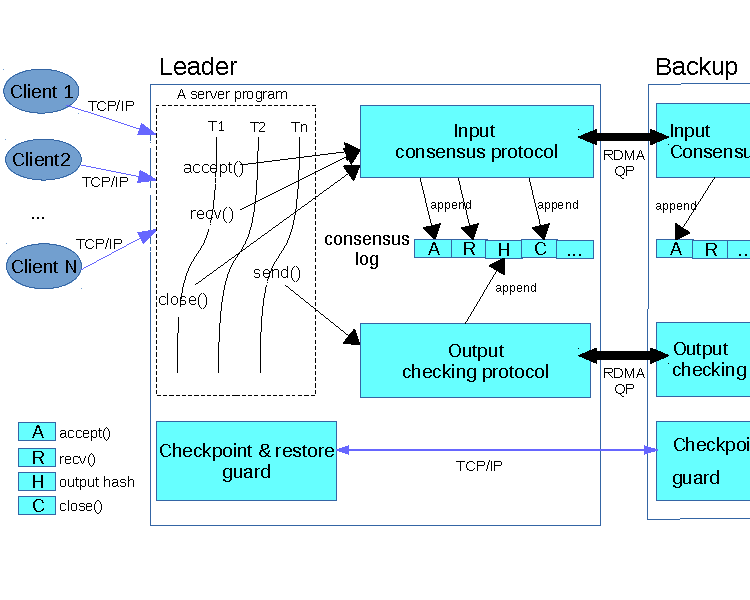
\includegraphics[width=.5\textwidth]{figures/arch}
\vspace{-.20in}
\caption{{\em The \xxx Architecture.} \xxx components are shaded (and in
  green).} \label{fig:arch}
\vspace{-.05in}
\end{figure}

% \begin{figure*}[!htb]
% \centering
% 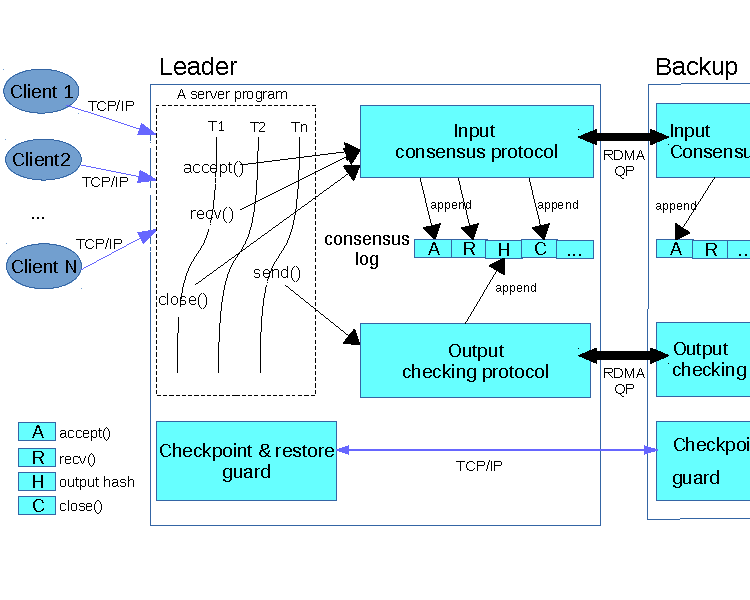
\includegraphics[width=0.5\textwidth]{figures/arch}
% \vspace{-.10in}
% \caption{{\em The \xxx Architecture.} \rm {\xxx components are shaded (and in
%   green).}} \label{fig:arch}
% \vspace{-.05in}
% \end{figure*}

% TBD. Input coordinator and output checker. Components.

% System model. Replicas. RDMA. LAN. Clients.
To replicate a server program, \xxx is deployed in a datacenter, with a set of 
three or five replicas connecting with RDMA architecture, InfiniBand. Client 
programs located in LAN or WAN network and send client requests to the leader 
machine as if only one server program is running. If clients send requests to 
the wrong machines, \xxx's backup machines deny the requests and reply the 
leader's IP.

% \xxx intercepts four types of 
% socket operations: the \accept type, the \recv type, the \send type, and the 
% \close type. 
Figure~\ref{fig:arch} shows \xxx's architecture within one replica machine. To 
run a server's x86 binary in a replica, \xxx simply runs this command: 
``LD\_PRELOAD=falcon.so ./server". \xxx invokes a server program's socket calls 
(\eg, \recv) and involve four key components: the input coordination 
protocol (for short, \emph{coordinator}), the output checking protocol (the 
\emph{checker}), the in-memory consensus log (the \emph{log}), the guard process 
that handles checkpointing and recovering the process state and file system 
state of the server program (the \emph{guard}).



% Coordinator: leader side. 
The coordinator is invoke when a server's thread calls a socket call to 
accept/close a client socket connection or to receive input bytes from the 
connection. On the leader replica, \xxx executes the actual Libc socket 
call, extracts the returned contents of this call (\eg, the returned buffer 
from \recv), and invokes the coordinator for a new consensus request on this 
socket call with the contents. Sending consensus request is fast because the 
leader coordinator directly writes a socket call request to remote backup 
replicas' log with RDMA. In this request, in order tell the backups what socket 
calls they should execute, this request also carries the latest request 
viewstamp that has reached consensus (\ie, the latest committed request).

% This coordinator invokes a consensus request by: (1) assigns this call a 
% monotonically increasing index (\ie, a viewstamp) in the log, (2) builds a 
% socket call struct (\S\ref{sec:input}), (3) store the struct to persistent 
% storage, (4) appends it to the log according to the index, and (5) writes this 
% struct to all remote backup replicas' log.

% Coordinator: backup side.
On a backup replica, \xxx's coordinator check its own log to receive new 
consensus requests, and it directly sends an Yes or No ACK by writing the 
remote leader's same struct for this socket call with RDMA. The backup 
coordinator then forwards all the requests up to the latest committed socket 
call to its local server process. \xxx does not need to intercept a 
server's socket calls in backups because these servers just follow the 
leader's consensus requests. To respond consensus requests rapidly, each 
backup coordinator spawns a dedicated thread. This thread runs a busy loop to 
pull consensus requests from the consensus log. This high-perfomance thread 
runs in a spare dedicated CPU core and elinimates context switches, unlike 
traditional TCP/IP that block threads socket calls to wait for requests.

% Consensus log. Same in both leader and backups.
A consensus log appending operation is invoked whenever a leader's server 
executes a socket call (except \send calls, handled by output checker). The 
leader coordinator just appends socket calls to the log and backups follow 
socket calls in this log.

% Output checker: leader side. % Output checker: backup side.
Output checker is occasionally invoked as the leader's server program executes 
\send operations. For every 4K bytes (MTU size) of output in each connection, 
the checker unions the current hash with these bytes and computes a new hash. 
Then, for every \emph{Tcheck} hash generations, the checker invokes a consensus 
request on this hash value. This output consensus is the same as the 
coordinator's input consensus except that backups' output checkers send ACKs 
with their own hash values with the same index, whenever the hash values are 
ready (some backups may run slowly). When a majority of hashes are back, the 
leader's output checker compares these values and then makes an effort to roll 
back divergent replicas to a previous checkpoint before the last matching hash. 
The leader's checker rolls back other replicas by sending roll-back requests to 
the local guard.

% Guard: leader side. % Guard: backup sides.
% Question: how does the backup replicas know the last matching hash? Through 
% committed viewstamp for the \send.
The leader's guard accepts roll-back requests from the output checker and 
forwards the requests to the corresponding guard on another, divergent repilca. 
The divergent replca's guard then rolls back the server program to a previous 
checkpoint before the last matching one, and then invokes the local input 
coordinator to re-forward the requests in stable storage to the server. There 
is no a second output hash comparisons between backups and leader until the 
leader invokes a new output checking consensus request next time.


\subsection{\xxx Has Broad Applications}\label{sec:apps}

We envision that \xxx's a fast, general SMR service can be applied in broad 
areas, and here we elaborate three. First, \xxx's RDMA-accelerated \paxos 
protocol and its implementation could be an effective template for many other 
distributed protocols in datacenters. For instance, an immediate extension of 
\xxx is to make it tolerate byzantine faults. Another promising direction is 
three-phase commit (3PC): 3PC is often blamed by its intolerance on network 
partitions and asynchronour communications, and its high latency caused by the 
three round-trips. Fortunately, within the RDMA-enabled datacenter context, 
people may leverage \xxx's techniques and experience to build a significantly 
faster and more reliable 3PC protocols.

% Other replication topics.

% Parallel program analysis. Such a short coordination time can make replicas 
% run almost as fast as each other, support many time-critical analyses 
% such as race detection and security defenses.
Second, by efficiently constructing multiple, equivalent executions for the 
same program, \xxx can benefit distributed program analysis techniques. Bounded 
by the limited computing resources on single machine, recent advanced 
reliability and security analaysis frameworks are moving towards distributed in 
order to offload analyses on multiple machines. \xxx can be leveraged in these 
frameworks so that developers of analysis tools can just focus on their own 
analysis logic, while \xxx's general replication architecture efficiently 
handles the rest. Moreover, analyses developers can tightly integrate their 
tools with \xxx (\eg, they can proactively diversify the orders of socket 
calls in \xxx's consensus logs among replicas to improve replicas' tolerance on
security attacks).

% TBD: use \xxx to detect software bugs by checking outputs, even in 
% real-world deployments. XXX make program % inputs strongly consistent across 
% replicas, so output divergence are likely % from software bugs. XXX promising 
% 
% results in our evaluation. Find a bug in % ssdb?

% One idea: can leverage the checkpoint and rollback protocok, and the 
% consensus part, to build a system that can automatically bypass concurrency 
% bugs without fixing them. The way to bypass: proactively reordering socket 
% calls. Self-healing system.

% A core building block in future operating systems. Maintain a consistent view 
% of computing resources and data. Used in scheduling framework (Mesos) because 
% its latency is almost compatible with context switches of processes (sub 
% milli seconds).
Third, \xxx can be a core building block in the emerging datacenter operating 
systems~\cite{hotos15, mesos, web-article}. As a datacenter continuously 
emerges a computer, an OS may be increasingly needed for thus a giant 
computer. \xxx's fast, general coordination service is espeicially suitable 
for such an OS's scheduler to maintain a consistent, reliable view on both 
computing resources and data in a datacenter. For instance,, \xxx's latency is 
largely between 15 to 20 \us, much smaller than a typical context swtich of a 
process (typically, a few hundreds \us).

% \subsection{Example}\label{sec:example}
% 
% \begin{figure}[t]
% \centering
% \begin{minipage}{.5\textwidth}
% \lgrindfile{code/example.cpp.lineno}
% \end{minipage}
% \vspace{-.1in}
% \caption{{\em A server example.}} \label{fig:example}
% \vspace{-.20in}
% \end{figure}
% 
% \begin{figure}[t]
% \centering
% \begin{minipage}{.5\textwidth}
% \lgrindfile{code/client.cpp.lineno}
% \end{minipage}
% \vspace{-.1in}
% \caption{{\em A client example.}} \label{fig:client}
% \vspace{-.05in}
% \end{figure}

% TBD. A simple server with recv(), accept(), and send(). Must have a 
% concurrency bug in this toy program? Race on global var or heap?

% Describe the example code.
% Describe the example code. Describe a 'set' command from key-value store.
% Figure~\ref{fig:example} shows a simplified server code based on the \redis 
% key-value store, and Figure~\ref{fig:client} shows a client cocde. The server 
% accepts a new connection from a client, receives one input request, process the 
% request, and then sends a reply. Suppose the client sends a ``SET a b" request.

% Input coordination protocol.
% Once the client calls its \connect, the leader's server program calls the 
% \accept call intercepted by \xxx. The leader's input coordinator then invokes 
% consensus on building a new connection by writing a struct for \accept to 
% remote backups with RDMA. Once a majority of backups agree, the leader machine 
% returns from the \accept call and continues to run.

% When a client program calls its \send, leader's server traps into \xxx's \recv 
% function call, which a invokes consensus on this new input ``SET a b". If 
% a consensus is made by a majority of replicas, the leader directly returns from 
% \recv and processes the request, and each replica's dedicated thread sets up 
% a new connection to the local server because the \recv consensus request 
% notifies the backups that the last call, \accept, has reached consensus.


% Output checking protcol.
% Challenge: what if leader does more sends and replicas do fewer sends?
% When a request is processed and the server is about to send reply to the 
% client, \xxx traps into the \send call, computes historical hash value on 
% inputs when 4K bytes (MTU size). Since this request is short, no output check 
% will be invoked at this time. All backups return consensus reply to the leader 
% with their own hash values if this value is available on their replica. 
% Similarly, backups do the earlier socket call: the backups' follower forwards 
% ``SET a b" request to the local server program.

% TBD: explain why we do not need to intercept poll() function.

% TBD Question: must ask Cheng. The close logic is not clear. What do the 
% leaders and backups do for close()? Why do we have to need a NOP (if 
% backup thread does not close its connection to local server, it does not 
% matter, right)? 
% Finally, the leader's server program executes a \close call. Similarly, the 
% leader invokes consensus on this call, and the backups have this \close call in 
% their log so that they can close the 

% TBD: what is the interesting outcome of this program running with Falcon? 
% Replicating all inputs without modifications? Any chart figure/schedule? 
% Two points so far: automatically replicating all inputs without modification; 
% can tolerate one replica failure; the other two can still process requests.